% Options for packages loaded elsewhere
\PassOptionsToPackage{unicode}{hyperref}
\PassOptionsToPackage{hyphens}{url}
%
\documentclass[
]{book}
\usepackage{amsmath,amssymb}
\usepackage{iftex}
\ifPDFTeX
  \usepackage[T1]{fontenc}
  \usepackage[utf8]{inputenc}
  \usepackage{textcomp} % provide euro and other symbols
\else % if luatex or xetex
  \usepackage{unicode-math} % this also loads fontspec
  \defaultfontfeatures{Scale=MatchLowercase}
  \defaultfontfeatures[\rmfamily]{Ligatures=TeX,Scale=1}
\fi
\usepackage{lmodern}
\ifPDFTeX\else
  % xetex/luatex font selection
\fi
% Use upquote if available, for straight quotes in verbatim environments
\IfFileExists{upquote.sty}{\usepackage{upquote}}{}
\IfFileExists{microtype.sty}{% use microtype if available
  \usepackage[]{microtype}
  \UseMicrotypeSet[protrusion]{basicmath} % disable protrusion for tt fonts
}{}
\makeatletter
\@ifundefined{KOMAClassName}{% if non-KOMA class
  \IfFileExists{parskip.sty}{%
    \usepackage{parskip}
  }{% else
    \setlength{\parindent}{0pt}
    \setlength{\parskip}{6pt plus 2pt minus 1pt}}
}{% if KOMA class
  \KOMAoptions{parskip=half}}
\makeatother
\usepackage{xcolor}
\usepackage{color}
\usepackage{fancyvrb}
\newcommand{\VerbBar}{|}
\newcommand{\VERB}{\Verb[commandchars=\\\{\}]}
\DefineVerbatimEnvironment{Highlighting}{Verbatim}{commandchars=\\\{\}}
% Add ',fontsize=\small' for more characters per line
\usepackage{framed}
\definecolor{shadecolor}{RGB}{248,248,248}
\newenvironment{Shaded}{\begin{snugshade}}{\end{snugshade}}
\newcommand{\AlertTok}[1]{\textcolor[rgb]{0.94,0.16,0.16}{#1}}
\newcommand{\AnnotationTok}[1]{\textcolor[rgb]{0.56,0.35,0.01}{\textbf{\textit{#1}}}}
\newcommand{\AttributeTok}[1]{\textcolor[rgb]{0.13,0.29,0.53}{#1}}
\newcommand{\BaseNTok}[1]{\textcolor[rgb]{0.00,0.00,0.81}{#1}}
\newcommand{\BuiltInTok}[1]{#1}
\newcommand{\CharTok}[1]{\textcolor[rgb]{0.31,0.60,0.02}{#1}}
\newcommand{\CommentTok}[1]{\textcolor[rgb]{0.56,0.35,0.01}{\textit{#1}}}
\newcommand{\CommentVarTok}[1]{\textcolor[rgb]{0.56,0.35,0.01}{\textbf{\textit{#1}}}}
\newcommand{\ConstantTok}[1]{\textcolor[rgb]{0.56,0.35,0.01}{#1}}
\newcommand{\ControlFlowTok}[1]{\textcolor[rgb]{0.13,0.29,0.53}{\textbf{#1}}}
\newcommand{\DataTypeTok}[1]{\textcolor[rgb]{0.13,0.29,0.53}{#1}}
\newcommand{\DecValTok}[1]{\textcolor[rgb]{0.00,0.00,0.81}{#1}}
\newcommand{\DocumentationTok}[1]{\textcolor[rgb]{0.56,0.35,0.01}{\textbf{\textit{#1}}}}
\newcommand{\ErrorTok}[1]{\textcolor[rgb]{0.64,0.00,0.00}{\textbf{#1}}}
\newcommand{\ExtensionTok}[1]{#1}
\newcommand{\FloatTok}[1]{\textcolor[rgb]{0.00,0.00,0.81}{#1}}
\newcommand{\FunctionTok}[1]{\textcolor[rgb]{0.13,0.29,0.53}{\textbf{#1}}}
\newcommand{\ImportTok}[1]{#1}
\newcommand{\InformationTok}[1]{\textcolor[rgb]{0.56,0.35,0.01}{\textbf{\textit{#1}}}}
\newcommand{\KeywordTok}[1]{\textcolor[rgb]{0.13,0.29,0.53}{\textbf{#1}}}
\newcommand{\NormalTok}[1]{#1}
\newcommand{\OperatorTok}[1]{\textcolor[rgb]{0.81,0.36,0.00}{\textbf{#1}}}
\newcommand{\OtherTok}[1]{\textcolor[rgb]{0.56,0.35,0.01}{#1}}
\newcommand{\PreprocessorTok}[1]{\textcolor[rgb]{0.56,0.35,0.01}{\textit{#1}}}
\newcommand{\RegionMarkerTok}[1]{#1}
\newcommand{\SpecialCharTok}[1]{\textcolor[rgb]{0.81,0.36,0.00}{\textbf{#1}}}
\newcommand{\SpecialStringTok}[1]{\textcolor[rgb]{0.31,0.60,0.02}{#1}}
\newcommand{\StringTok}[1]{\textcolor[rgb]{0.31,0.60,0.02}{#1}}
\newcommand{\VariableTok}[1]{\textcolor[rgb]{0.00,0.00,0.00}{#1}}
\newcommand{\VerbatimStringTok}[1]{\textcolor[rgb]{0.31,0.60,0.02}{#1}}
\newcommand{\WarningTok}[1]{\textcolor[rgb]{0.56,0.35,0.01}{\textbf{\textit{#1}}}}
\usepackage{longtable,booktabs,array}
\usepackage{calc} % for calculating minipage widths
% Correct order of tables after \paragraph or \subparagraph
\usepackage{etoolbox}
\makeatletter
\patchcmd\longtable{\par}{\if@noskipsec\mbox{}\fi\par}{}{}
\makeatother
% Allow footnotes in longtable head/foot
\IfFileExists{footnotehyper.sty}{\usepackage{footnotehyper}}{\usepackage{footnote}}
\makesavenoteenv{longtable}
\usepackage{graphicx}
\makeatletter
\newsavebox\pandoc@box
\newcommand*\pandocbounded[1]{% scales image to fit in text height/width
  \sbox\pandoc@box{#1}%
  \Gscale@div\@tempa{\textheight}{\dimexpr\ht\pandoc@box+\dp\pandoc@box\relax}%
  \Gscale@div\@tempb{\linewidth}{\wd\pandoc@box}%
  \ifdim\@tempb\p@<\@tempa\p@\let\@tempa\@tempb\fi% select the smaller of both
  \ifdim\@tempa\p@<\p@\scalebox{\@tempa}{\usebox\pandoc@box}%
  \else\usebox{\pandoc@box}%
  \fi%
}
% Set default figure placement to htbp
\def\fps@figure{htbp}
\makeatother
\setlength{\emergencystretch}{3em} % prevent overfull lines
\providecommand{\tightlist}{%
  \setlength{\itemsep}{0pt}\setlength{\parskip}{0pt}}
\setcounter{secnumdepth}{5}
\usepackage{booktabs}
\usepackage{setspace}
%\usepackage{amsthm}
%\usepackage{ltxdoc}
%\usepackage{amsthm}

%\makeatletter
%\def\thm@space@setup{%
%  \thm@preskip=8pt plus 2pt minus 4pt
%  \thm@postskip=\thm@preskip
%}
%\makeatother

% ==== Math (classic stack; no unicode-math) ====
\usepackage{amsmath,amssymb,bm,mathtools}
% If you use theorem environments:
\usepackage{amsthm}

% Bold symbols
\newcommand{\bs}[1]{\boldsymbol{#1}}  % wrapper
\newcommand{\bsm}{\bs{m}}
\newcommand{\balpha}{\bs{\alpha}}
\newcommand{\bp}{\bs{p}}
\newcommand{\bbeta}{\bs{\beta}}

% Sets/simplex
\newcommand{\IN}{\mathbb{N}}
\newcommand{\IR}{\mathbb{R}}
\newcommand{\simp}{\Delta}

% Operators
\DeclareMathOperator{\E}{\mathbb{E}}
\DeclareMathOperator{\Var}{Var}
\DeclareMathOperator{\Prb}{Pr}   % use \Prb to avoid clashes; or \Pr if unused elsewhere

% Transpose
\newcommand{\trans}{^{\mathsf T}}

% Distribution shorthands (as text inside math)
\newcommand{\DM}{\mathrm{DM}}
\newcommand{\Dir}{\mathrm{Dir}}
\newcommand{\Mult}{\mathrm{Multinomial}}
\usepackage[]{natbib}
\bibliographystyle{plainnat}
\usepackage{bookmark}
\IfFileExists{xurl.sty}{\usepackage{xurl}}{} % add URL line breaks if available
\urlstyle{same}
\hypersetup{
  pdftitle={Advanced Research Writing in Statistics and Data Science},
  pdfauthor={Kun Chen, Elizabeth Schifano, Jun Yan},
  hidelinks,
  pdfcreator={LaTeX via pandoc}}

\title{Advanced Research Writing in Statistics and Data Science}
\author{Kun Chen, Elizabeth Schifano, Jun Yan}
\date{2025-08-22}

\usepackage{amsthm}
\newtheorem{theorem}{Theorem}[chapter]
\newtheorem{lemma}{Lemma}[chapter]
\newtheorem{corollary}{Corollary}[chapter]
\newtheorem{proposition}{Proposition}[chapter]
\newtheorem{conjecture}{Conjecture}[chapter]
\theoremstyle{definition}
\newtheorem{definition}{Definition}[chapter]
\theoremstyle{definition}
\newtheorem{example}{Example}[chapter]
\theoremstyle{definition}
\newtheorem{exercise}{Exercise}[chapter]
\theoremstyle{definition}
\newtheorem{hypothesis}{Hypothesis}[chapter]
\theoremstyle{remark}
\newtheorem*{remark}{Remark}
\newtheorem*{solution}{Solution}
\begin{document}
\maketitle

{
\setcounter{tocdepth}{1}
\tableofcontents
}
\chapter*{Preface}\label{preface}
\addcontentsline{toc}{chapter}{Preface}

This book aims to train students in statistics and data science on academic
writing with professional tools such as LaTeX, BibTeX, R, and Git.

This book is currently under-development, and it is meant to be
an extended version of the book ``Statistical Writing'' \url{https://github.com/statds/stat-writing} written by Dr.~Elizabeth Schifano and Dr.~Jun Yan.

The notes are prepared with the \textbf{bookdown} R package \citep{xie2016bookdown},
which can be installed from CRAN or Github:

\begin{Shaded}
\begin{Highlighting}[]
\FunctionTok{install.packages}\NormalTok{(}\StringTok{"bookdown"}\NormalTok{)}
\CommentTok{\# or the development version}
\CommentTok{\# devtools::install\_github("rstudio/bookdown")}
\end{Highlighting}
\end{Shaded}

Remember each Rmd file contains one and only one chapter, and a chapter is
defined by the first-level heading \texttt{\#}.

To compile this example to PDF, you need XeLaTeX. You are recommended to install
TinyTeX (which includes XeLaTeX): \url{https://yihui.name/tinytex/}.

\chapter{Introduction}\label{intro}

What does a statistical or data science paper look like? As with all scientific papers, it should have some commonly expected structures: title, abstract, keywords, introduction, methods, results, discussion, acknowledgements, references, appendix, and supplement. Due to the specificity of the statistical discipline, machine learning practices, and application domains, however, research papers can look very different from one another.

What does a statistical or data science paper look like, and why should we study it?\\
For many graduate students and researchers, writing a paper is one of the most challenging yet most important parts of their training. A paper is more than just record of results; correctness is only the bottom line. A paper is the primary way for researchers to communicate ideas, establish credibility, and contribute to scientific literature. Good writing makes research visible, while poor writing may jeopardize delay the acknowledgement of even the most important discoveries.

As with all scientific papers, statistical and data science articles generally follow a set of commonly expected structures: title, abstract, keywords, introduction, methods, results, discussion, acknowledgements, references, appendix, and supplement. Yet, due to the specificity of the statistical discipline, the practices of machine learning, and the variety of application domains, research papers can look very different from one another.

This book (and its companion course) is motivated by the need to make these conventions explicit, to demystify the writing process, and to provide practical guidance through many examples and exercises. It is designed for graduate students and researchers who wish to sharpen their writing, whether they are preparing a dissertation chapter, a methodological paper, or an applied paper. Our goal is to teach students \emph{how} statistical and data science papers are structured, \emph{why} they are written in such ways, and \emph{what} we shall do to adapt writing for different audiences and outlets.

\begin{center}\rule{0.5\linewidth}{0.5pt}\end{center}

\section{Types of Papers in Statistics and Data Science}\label{types-of-papers-in-statistics-and-data-science}

\subsection{Theory papers}\label{theory-papers}

A \textbf{theory paper} in statistics and probability is closest in form to a mathematical paper. It typically includes the statement of the problem, formulation of assumptions, and the presentation of theorems, lemmas, and proofs. The purpose is often to establish fundamental properties of certain statistical or probabilistic tools/approaches, including but well beyond consistency, efficiency, optimality, convergence, asymptotic distributions, and non-asymptotic error bounds.

While theory papers may not always feature data, simulations, or applications, they form the \textbf{mathematical and probabilistic foundation} upon which methodology and applied work are built.

Most of the articles in journals such as \emph{Annals of Statistics}, \emph{Annals of Probability}, \emph{Bernoulli}, \emph{Probability Theory and Related Fields}, among others, are considered as theory papers. In other words, these journals should be the primary outlets for a theory paper.

Examples include \citet{Foygel2021}.

\subsection{Methodological papers}\label{methodological-papers}

A \textbf{methodological paper} focuses on proposing a novel methodological contribution that can be applied to a general class of real-world problems. A commonly seen structure is:

\begin{itemize}
\tightlist
\item
  Introduction
\item
  Literature review
\item
  Methods (e.g., estimation, hypothesis tests, diagnostic procedures)\\
\item
  Theoretical properties\\
\item
  Simulation studies\\
\item
  Applications/Illustrations\\
\item
  Discussion/Conclusions
\end{itemize}

Such papers emphasis on methodological development, with a blend of theory (e.g., asymptotic or non-asymptotic guarantees) and empirical validations.

Such papers emphasize methodological development, often with a blend of theory (e.g., asymptotic or non-asymptotic guarantees) and empirical validations. Astrong methodological paper should not be just a mechanical combination or minor extension of existing methods. Instead, it should be driven by a clear motivation from real-world applications.

In other words, the most impactful methodological contributions are those that connect with practical relevance. They are inspired by genuine applied needs, but provide solutions that are general enough to influence future work in an important domain or even across different domains.

Example include \citet{li2023regularized} and \citet{lau2022bias}.

\subsection{Applied papers}\label{applied-papers}

An \textbf{applied paper} focuses on addressing a concrete scientific question in a particular domain using statistical or data science methods. Its structure often includes:

\begin{itemize}
\tightlist
\item
  Introduction\\
\item
  Data description\\
\item
  Methods (applied or adapted)\\
\item
  Results\\
\item
  Discussion
\end{itemize}

Sometimes simulation studies are added to assess sensitivity. Applied papers may involve applying existing methods or developing new ones motivated by the application. Examples include \citet{price2022effects}; \citet{caplan2019dental}; \citet{jiao2022cyberattack}.

It is important to note that what we call ``applied papers'' here includes a large portion of scientific papers that rely on data analytics, statistics, and machine learning methods. In many scientific domains, these papers may in fact be considered theoretical or methodological contributions within that field. For instance, an applied paper with genomical data analysis could be regarded as a methodological paper in genetics.

Such works are most often interdisciplinary, typically resulting from close collaborations between statisticians, data scientists, and domain experts. They showcase how quantitative methods advance science in other fields, while also motivating the development of new techniques within statistics and machine learning.

\begin{center}\rule{0.5\linewidth}{0.5pt}\end{center}

\subsection{Data Science and Machine Learning Papers}\label{data-science-and-machine-learning-papers}

Beyond traditional statistics journals, researchers often publish in data science, machine learning, and data mining journals and conferences, including outlets such as \emph{NeurIPS}, \emph{ICML}, \emph{KDD}, and \emph{AAAI}. These conference papers emphasize:

\begin{itemize}
\tightlist
\item
  Conciseness (strict page limits)\\
\item
  Algorithmic novelty\\
\item
  Benchmark comparisons on standard datasets\\
\item
  Open-source reproducibility\\
\item
  Clarity for an interdisciplinary readership
\end{itemize}

Compared to \emph{JASA} or \emph{Annals of Statistics}, these outlets often prioritize empirical performance and novelty over extensive theoretical justifications or methodological development, though many still include core mathematical or probabilistical analysis. This emphasis partly reflects the nature of the research topics: for many cutting-edge machine learning and AI methods, their theoretical understanding is still evolving and often lags behind practice. As a result, papers are judged primarily on their ability to demonstrate empirical advances on benchmark datasets or practical applications.

\begin{center}\rule{0.5\linewidth}{0.5pt}\end{center}

\section{Scientific Writing Resources}\label{scientific-writing-resources}

Many resources on scientific writing are available. For example, \citet{gopen1990science} was selected by its publisher, \emph{American Scientist}, as one of its 36 ``Classic Articles'' from the first 100 years of publishing history. Popular books are \citet{oshima2000writing}, \citet{gopen2004expectations}, \citet{hairston2003successful}, and \citet{lebrun2021scientific}.

\begin{center}\rule{0.5\linewidth}{0.5pt}\end{center}

\section{About This Book}\label{about-this-book}

This book, \emph{Advanced Research Writing in Statistics and Data Science}, extends earlier efforts from \href{https://statds.github.io/stat-writing/}{\emph{Statistical Writing}}, by broadening its scope and including hands-on examples and exercises.

The book emphasizes three guiding principles:

\begin{enumerate}
\def\labelenumi{\arabic{enumi}.}
\item
  \textbf{Clarity}: communicating complex technical ideas to both expert and interdisciplinary audiences.
\item
  \textbf{Adaptivity}: tailoring style and structure to journals, conferences, and other outlets.\\
\item
  \textbf{Learning by Doing}: the book includes examples, annotated excerpts, and practical exercises.
\end{enumerate}

\begin{center}\rule{0.5\linewidth}{0.5pt}\end{center}

\section{Outline of the Book}\label{outline-of-the-book}

The planned content includes:

\begin{itemize}
\tightlist
\item
  \textbf{Introduction} (this chapter): Types of research papers --- theory, methods, and applied --- and the conventions of scientific writing across statistics, data science, and machine learning.\\
\item
  \textbf{Tools and Workflows for Writing}: Version control (Git/GitHub), LaTeX, R Markdown/Bookdown, and reproducibility practices.\\
\item
  \textbf{Getting Started with Writing}: The research and writing lifecycle, writing proposals, and planning strategies.\\
\item
  \textbf{Writing Specific Sections}: Titles, abstracts, introductions, methods, results, discussion, figures, tables, captions, and style.\\
\item
  \textbf{Writing for Different Outlets}: How to adapt writing for different audiences and venues --- e.g., writing statistical analysis sections in interdisciplinary papers, preparing concise ML/AI conference papers, and meeting expectations in statistics journals.\\
\item
  \textbf{Peer Review and Revision}: How to review manuscripts constructively, write referee reports, and respond to reviewers effectively.\\
\item
  \textbf{Grant Proposals and Research Statements}: Writing for funding agencies, fellowships, and academic job applications.\\
\item
  \textbf{Ethics and Integrity}: Authorship, plagiarism, collaboration, and responsible use of AI tools.\\
\item
  \textbf{Exercises and Practice}: Rewriting, reviewing, and polishing tasks, designed to simulate authentic writing and reviewing experiences.
\end{itemize}

Each chapter will include \textbf{examples drawn from real papers across statistics, biostatistics, and machine learning} and will feature \textbf{exercises} that encourage hands-on practice and reflection.

\begin{center}\rule{0.5\linewidth}{0.5pt}\end{center}

\section{Before We Start}\label{before-we-start}

An author should always keep the target audience in mind. Statistical journals span a wide spectrum from applied to theoretical. Machine learning venues differ again in expectations. Even technical reports, white papers, or grant proposals have unique readerships.

Regardless of outlet, any scientific writing should be convincing and concise. Authors need to show clearly that their work is important, valid, and useful.

Ultimately, strong writing can never substitute for strong research. In short, keep in mind that \textbf{a good paper must rest on good work}. Just as important, a good paper is made through revision.

Or, as the Chinese phrase puts it: \textbf{好文章是改出来的}.

You can view an example of a marked-up draft with comments from my PhD advisor:\\
\href{files/ks-comments.pdf}{Download advisor's comments (PDF)}

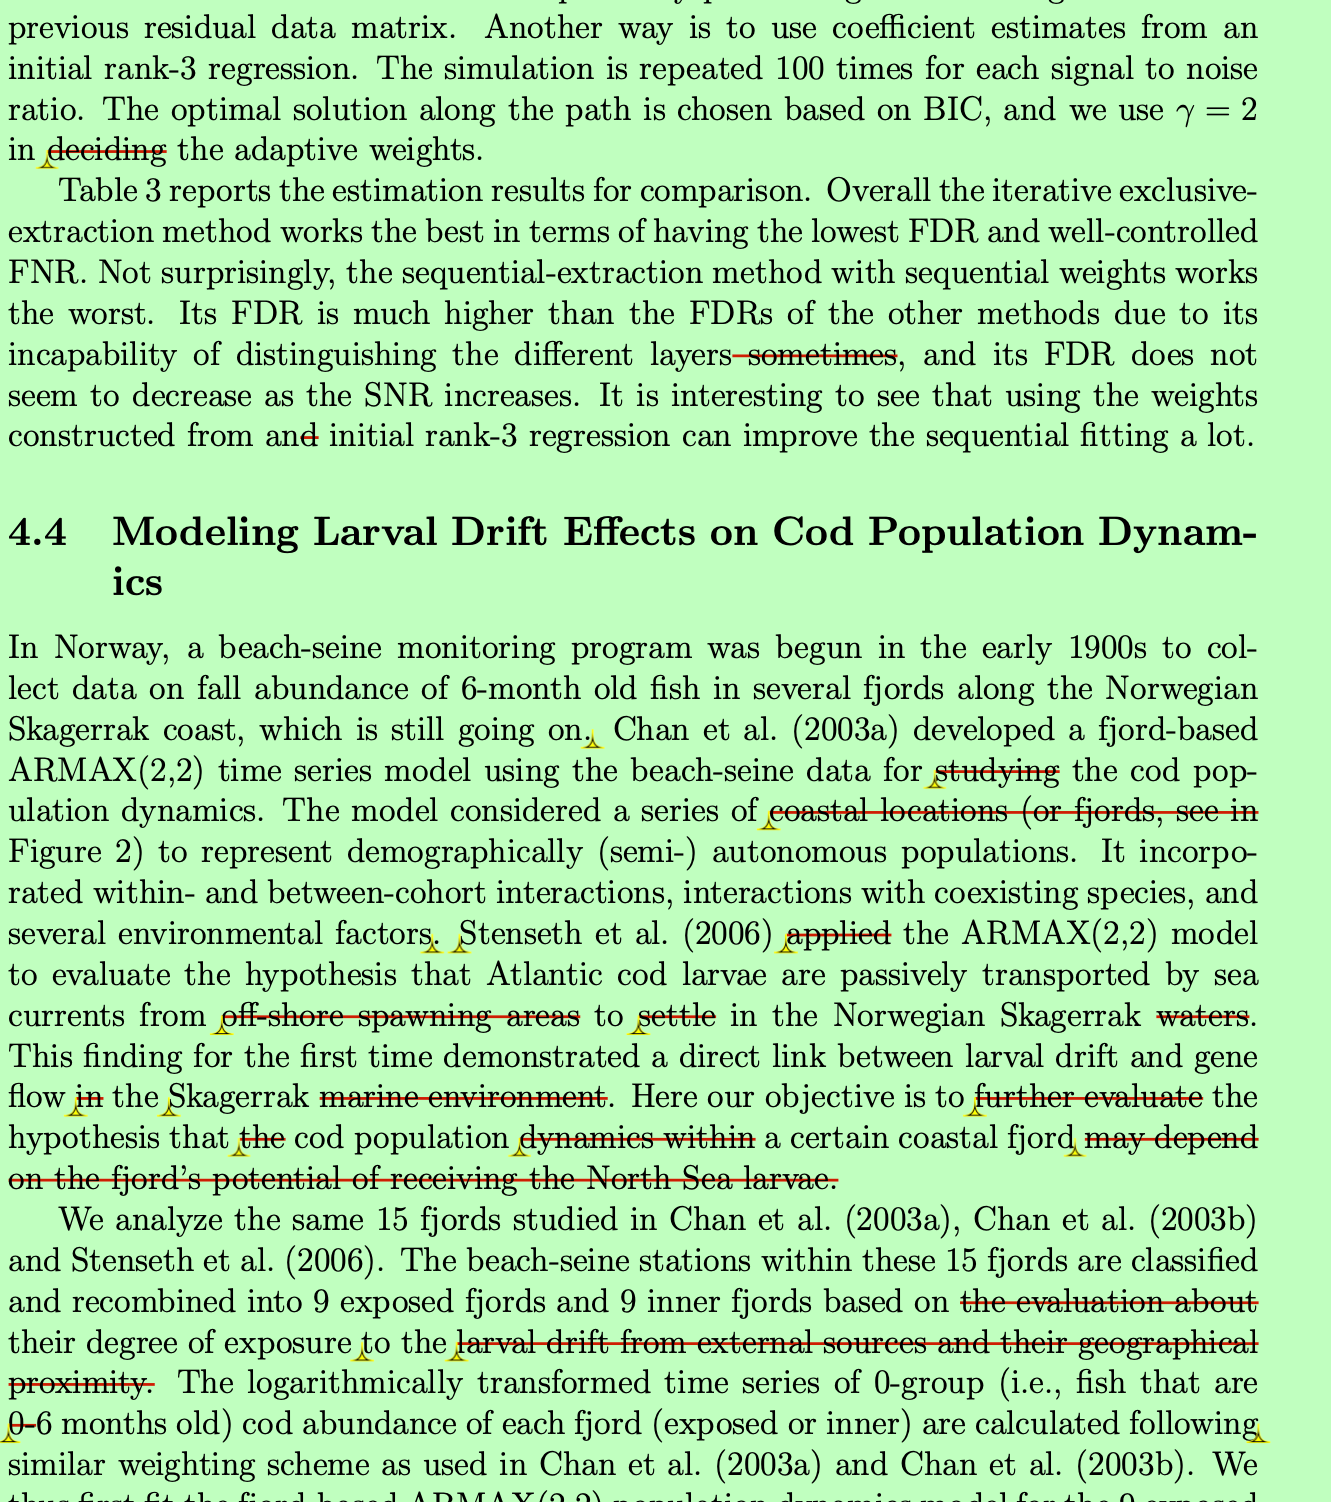
\includegraphics[width=0.7\linewidth,height=\textheight,keepaspectratio]{files/ks-comments.png}

\begin{center}\rule{0.5\linewidth}{0.5pt}\end{center}

\chapter{Tools and Workflows for Writing}\label{ch-tools}

Many people use MS Word when it comes to writing.
Not withholding the importance of the invention of MS Office, it is not the right tool to write methodological or theoretical papers in
statistics. To many, writing a statistical
paper using MS Word would be as interesting as running a statistical data
analysis using MS Excel. Simply put, MS Office is great for office staff to do
routine office documentary tasks.

For professional writing, one need to be aware
of the professional tools and invest time to master them.

\begin{center}\rule{0.5\linewidth}{0.5pt}\end{center}

\section{Word vs.~LaTeX}\label{word-vs.-latex}

The right, high - quality, professional typesetting system is LaTeX. LaTeX is a
typesetting language that makes it easier and cleaner to write documents
involving extensive mathematical content. It is the standard in Statistics, Mathematics, Physics, Chemistry and other disciplines that require many
mathematical formulas.

LaTeX separates the appearance of a document from its content. This allows authors
to be able to focus on writing the content without having to worry about
its appearance until the end. There are many different
professionally looking appearances one can choose or design, allowing for easy
adaptation to different formats and styles.

A LaTeX document has \texttt{.tex} extension, and can be
edited by your favorite text editor. The final output of the document can have
different formats, the most popular of which is \texttt{pdf}, which stands for \emph{
portable
document format } . It can be opened on any platform (computer operating system).

The source \texttt{.tex} file is a plain text file. Just like source code of any
programming language, a plain text file allows version control, which makes
tracking and managing the source easy and professional. The most popular version
control tool today is \texttt{git}.

\begin{example}
\textbf{LaTeX vs.~Word}

Suppose you want to write down a likelihood function for a Gaussian model:
\[
L(\mu, \sigma^2 \mid x_1, \ldots, x_n)= (2\pi\sigma^2)^{-n / 2}\exp\left\{
-\frac{1}{2\sigma^2}\sum_{i = 1}^n(x_i - \mu)^2\right\}.
\]

\begin{itemize}
\tightlist
\item
  \textbf{In LaTeX} , the source code is simple and transparent:
\end{itemize}

\begin{Shaded}
\begin{Highlighting}[]
\NormalTok{L(}\FunctionTok{\textbackslash{}mu}\NormalTok{, }\FunctionTok{\textbackslash{}sigma}\NormalTok{\^{}2 }\FunctionTok{\textbackslash{}mid}\NormalTok{ x\_1, }\FunctionTok{\textbackslash{}ldots}\NormalTok{, x\_n) = (2}\FunctionTok{\textbackslash{}pi\textbackslash{}sigma}\NormalTok{\^{}2)\^{}\{{-}n / 2\}}\FunctionTok{\textbackslash{}exp\textbackslash{}left\textbackslash{}\{}
\NormalTok{{-}}\FunctionTok{\textbackslash{}frac}\NormalTok{\{1\}\{2}\FunctionTok{\textbackslash{}sigma}\NormalTok{\^{}2\}}\FunctionTok{\textbackslash{}sum}\NormalTok{\_\{i = 1\}\^{}n(x\_i {-} }\FunctionTok{\textbackslash{}mu}\NormalTok{)\^{}2}\FunctionTok{\textbackslash{}right\textbackslash{}\}}\NormalTok{.}
\end{Highlighting}
\end{Shaded}

This produces beautifully typeset mathematics, is reproducible, and can be revised easily.
In MS Word, one must insert each symbol manually through the Equation Editor:Greek letters via dropdowns, summations via menus, exponents via special boxes. Formatting quickly becomes clumsy, and editing dozens of formulas is tedious. Copy-pasting often breaks structure, and version control is nearly impossible.

For one or two equations Word may be acceptable. But for an entire paper with dozens of equations,
cross-references, and theorems, LaTeX is the only tool that is professional, efficient, and sustainable.
\end{example}

\begin{exercise}

Compare Word and LaTeX

\begin{enumerate}
\def\labelenumi{\arabic{enumi}.}
\item
  Typeset the following equation in \textbf{MS Word} using its built - in Equation Editor:
  \[
  \hat{\beta} = \arg\min_{\beta \in \mathbb{R}^p}\left\{\frac{1}{2n}\ | y - X\beta\ | _2^2 + \lambda \ | \beta\ | _1 \right\}.
  \]
\item
  Now, paste this LaTeX code into Overleaf (or another LaTeX editor) and compile:
\end{enumerate}

\begin{Shaded}
\begin{Highlighting}[]
\FunctionTok{\textbackslash{}hat}\NormalTok{\{}\FunctionTok{\textbackslash{}beta}\NormalTok{\} = }\FunctionTok{\textbackslash{}arg\textbackslash{}min}\NormalTok{\_\{}\FunctionTok{\textbackslash{}beta} \FunctionTok{\textbackslash{}in} \FunctionTok{\textbackslash{}mathbb}\NormalTok{\{R\}\^{}p\}}
\FunctionTok{\textbackslash{}left\textbackslash{}\{\textbackslash{}frac}\NormalTok{\{1\}\{2n\}}\FunctionTok{\textbackslash{} }\NormalTok{| y {-} X}\FunctionTok{\textbackslash{}beta\textbackslash{} }\NormalTok{| \_2\^{}2 + }\FunctionTok{\textbackslash{}lambda} \FunctionTok{\textbackslash{} }\NormalTok{| }\FunctionTok{\textbackslash{}beta\textbackslash{} }\NormalTok{| \_1 }\FunctionTok{\textbackslash{}right\textbackslash{}\}}
\end{Highlighting}
\end{Shaded}

\begin{itemize}
\tightlist
\item
  Which approach is faster ?
\item
  Which result looks more professional ?
\item
  Which is easier to revise and share ?
\end{itemize}

\end{exercise}

While LaTeX is the professional standard for statistical and mathematical
writing, statisticians must also remain flexible when collaborating with
scientists from other fields. In many interdisciplinary projects, collaborators
still prefer Word as the common platform for writing and revision. This can also
often be the case when developing grant applications to
National Insititutes of Health (NIH).
This is understandable, since for papers in fileds such as biology, medicine, or social
sciences, statistical formulas are often minimal or should even be avoided
altogether. In such cases, it is often best to accommodate collaborators by
using Word for the main text, while reserving LaTeX for supplementary technical
sections, appendices, or internal drafts where precise mathematical notation is
required.

\begin{center}\rule{0.5\linewidth}{0.5pt}\end{center}

\section{Git for Version Control}\label{git-for-version-control}

Many tutorials are available in different formats. Here is a \href{https://www.youtube.com/watch?v=USjZcfj8yxE}{YouTube video
``Git and GitHub for Beginners---Crash
Course'\,'}.

The video also covers \href{https://github.com}{GitHub}, a cloud service for Git. Other similar services
are, for example, \href{https://bitbucket.org}{bitbucket} and \href{https://gitlab.com}{GitLab}. A cloud
service gives you a cloud back up of your work and makes collaboration with
co - workers easy.

There are tools and tutorials that make learning Git easy.

\begin{itemize}
\item
  Here is a collection of \href{https://gitexercises.fracz.com}{online Git exersices}
\item
  Here is a game called \href{https://ohmygit.org}{\texttt{Oh\ My\ Git}}, an open
  source game about learning Git!
\end{itemize}

\subsection{Set Up}\label{set-up}

\begin{itemize}
\item
  Download Git \href{https://git-scm.com/downloads}{here}.
\item
  Make a GitHub Account \href{https://www.github.com}{here} if you don't have one yet.
\item
  Get started with your GitHub account by following the \href{https://docs.github.com/en/get-started/onboarding/getting-started-with-your-github-account}{help
  page}.

  \begin{itemize}
  \item
    One important step is the
    \href{https://docs.github.com/en/get-started/onboarding/getting-started-with-your-github-account\#2-setting-up-git}{set-up}.
  \item
    The connection between your local and GitHub repositories needs
    to be \href{https://docs.github.com/en/get-started/getting-started-with-git/about-remote-repositories}{set up onlyonce}.
  \item
    One easy way is with a personal access token, as illustrated
    in a \href{https://www.youtube.com/watch?v=kHkQnuYzwoo}{YouTube video}.
  \end{itemize}
\end{itemize}

\subsection{Most Frequently Used Git Commands}\label{most-frequently-used-git-commands}

\begin{itemize}
\tightlist
\item
  \texttt{git\ clone}:

  \begin{itemize}
  \tightlist
  \item
    Clones a remote repository to a local folder.
  \item
    Requires either HTTPS link or SSH key to authenticate.
  \end{itemize}
\item
  \texttt{git\ pull}:

  \begin{itemize}
  \tightlist
  \item
    Downloads any updates made to the remote repository and automatically updates the local repository.
  \end{itemize}
\item
  \texttt{git\ status}:

  \begin{itemize}
  \tightlist
  \item
    Returns the state of the working directory.
  \item
    Lists the files that have been modified, and are yet to be or have been staged and/or committed.
  \item
    Shows if the local repository is begind or ahead a remote branch.
  \end{itemize}
\item
  \texttt{git\ add}:

  \begin{itemize}
  \tightlist
  \item
    Adds new or modified files to the Git staging area.
  \item
    Gives the option to select which files are to be sent to the remote repository.
  \end{itemize}
\item
  \texttt{git\ rm}:

  \begin{itemize}
  \tightlist
  \item
    Used to remove files from the staging index or the local repository.
  \end{itemize}
\item
  \texttt{git\ commit}:

  \begin{itemize}
  \tightlist
  \item
    Commits changes made to the local repository and saves it like a snapshot.
  \item
    A message is recommended with every commit to keep track of changes made.
  \end{itemize}
\item
  \texttt{git\ push}:

  \begin{itemize}
  \tightlist
  \item
    Pushes commits made on local repository to the remote repository.
  \end{itemize}
\end{itemize}

\begin{example}

\textbf{A clean daily Git workflow}

\begin{enumerate}
\def\labelenumi{\arabic{enumi}.}
\tightlist
\item
  Pull the latest changes
\end{enumerate}

\begin{Shaded}
\begin{Highlighting}[]
\FunctionTok{git}\NormalTok{ pull}
\end{Highlighting}
\end{Shaded}

\begin{enumerate}
\def\labelenumi{\arabic{enumi}.}
\setcounter{enumi}{1}
\item
  Write/edit files (e.g., intro.Rmd, style.css).
\item
  Check what has changed
\end{enumerate}

\begin{Shaded}
\begin{Highlighting}[]
\FunctionTok{git}\NormalTok{ status}
\FunctionTok{git}\NormalTok{ diff}
\end{Highlighting}
\end{Shaded}

\begin{enumerate}
\def\labelenumi{\arabic{enumi}.}
\setcounter{enumi}{3}
\tightlist
\item
  Stage only what you intend to commit
\end{enumerate}

\begin{Shaded}
\begin{Highlighting}[]
\FunctionTok{git}\NormalTok{ add intro.Rmd style.css}
\end{Highlighting}
\end{Shaded}

\begin{enumerate}
\def\labelenumi{\arabic{enumi}.}
\setcounter{enumi}{4}
\tightlist
\item
  Commit with a focused message
\end{enumerate}

\begin{Shaded}
\begin{Highlighting}[]
\FunctionTok{git}\NormalTok{ commit }\AttributeTok{{-}m} \StringTok{"intro: refine motivation; style: add callout color"}
\end{Highlighting}
\end{Shaded}

\begin{enumerate}
\def\labelenumi{\arabic{enumi}.}
\setcounter{enumi}{5}
\tightlist
\item
  Push to remote
\end{enumerate}

\begin{Shaded}
\begin{Highlighting}[]
\FunctionTok{git}\NormalTok{ push}
\end{Highlighting}
\end{Shaded}

\end{example}

\subsection{Tips on using Git:}\label{tips-on-using-git}

\begin{itemize}
\tightlist
\item
  Use the command line interface instead of the web interface (e.g., upload on GitHub)
\item
  Make frequent small commits instead of rare large commits.
\item
  Make commit messages informative and meaningful.
\item
  Name your files/folders by some reasonable convention.
\item
  Lower cases are better than upper cases.
\item
  No blanks in file/folder names.
\item
  Keep the repo clean by not tracking generated files.
\item
  Creat a \texttt{.gitignore} file for better output from \texttt{git\ status}.
\item
  Keep the linewidth of sources to under 80 for better \texttt{git\ diff} view.
\end{itemize}

\subsection{Pull Request}\label{pull-request}

To contribute to an open source project (e.g., our classnotes), use pull
requests. \href{https://docs.github.com/en/pull-requests/collaborating-with-pull-requests/proposing-changes-to-your-work-with-pull-requests/about-pull-requests}{Pull requests}
``let you tell others about changes you've pushed to a branch in a repository on
GitHub. Once a pull request is opened, you can discuss and review the potential
changes with collaborators and add follow-up commits before your changes are
merged into the base branch.''

Watch this YouTube video: \href{https://youtu.be/8lGpZkjnkt4}{GitHub pull requests in 100 seconds}.

\begin{example}
\textbf{A useful \texttt{.gitignore} for LaTeX/Bookdown}

Create a file named \texttt{.gitignore} in the project root:

\begin{Shaded}
\begin{Highlighting}[]
\NormalTok{\# RStudio }\OperatorTok{/}\NormalTok{ R files}
\NormalTok{.Rproj.}\FunctionTok{user}\OperatorTok{/}
\NormalTok{.Rhistory}
\NormalTok{.RData}
\NormalTok{.Ruserdata}

\NormalTok{\# Bookdown }\KeywordTok{build}\NormalTok{ output}
\NormalTok{\_book}\OperatorTok{/}
\NormalTok{\_bookdown\_files}\OperatorTok{/}
\OperatorTok{*}\NormalTok{.utf8.md}
\OperatorTok{*}\NormalTok{.knit.md}

\NormalTok{\# LaTeX }\KeywordTok{build}\NormalTok{ files}
\OperatorTok{*}\NormalTok{.aux}
\OperatorTok{*}\NormalTok{.bbl}
\OperatorTok{*}\NormalTok{.blg}
\OperatorTok{*}\NormalTok{.brf}
\OperatorTok{*}\NormalTok{.fls}
\OperatorTok{*}\NormalTok{.fdb\_latexmk}
\OperatorTok{*}\NormalTok{.idx}
\OperatorTok{*}\NormalTok{.ilg}
\OperatorTok{*}\NormalTok{.ind}
\OperatorTok{*}\NormalTok{.lof}
\OperatorTok{*}\NormalTok{.}\FunctionTok{log}
\OperatorTok{*}\NormalTok{.lot}
\OperatorTok{*}\NormalTok{.maf}
\OperatorTok{*}\NormalTok{.mtc}\OperatorTok{*}
\OperatorTok{*}\NormalTok{.}\KeywordTok{out}
\OperatorTok{*}\NormalTok{.pdf        \# }\OperatorTok{\textless{}}\CommentTok{{-}{-} if you want to keep generated PDFs out of git}
\OperatorTok{*}\NormalTok{.synctex.gz}
\OperatorTok{*}\NormalTok{.toc}
\OperatorTok{*}\NormalTok{.ttt}
\OperatorTok{*}\NormalTok{.xdv}

\NormalTok{\# Common OS junk}
\NormalTok{.DS\_Store}
\NormalTok{Thumbs.db}

\NormalTok{\# Editor files}
\OperatorTok{*}\NormalTok{.swp}
\OperatorTok{*}\NormalTok{.swo}
\end{Highlighting}
\end{Shaded}

Now \texttt{git\ status} will show only meaningful source changes.
\end{example}

\begin{center}\rule{0.5\linewidth}{0.5pt}\end{center}

\section{LaTeX}\label{latex}

\subsection{LaTeX Templates}\label{latex-templates}

A LaTeX source file has extension name \texttt{.tex}. It is a plain text file that can
be edited by any text editor. It can be tracked easily for differences between
any two versions. Different document classes are predefined such as \texttt{letter},
\texttt{article}, \texttt{report}, \texttt{beamer} (for presentations), and \texttt{book}. Customized
document classes can be defined once
you know more about LaTeX.

\begin{itemize}
\item
  The instructions in this section are practiced in a \href{https://github.com/jun-yan/writing-demo}{demo repo} from Professor Jun Yan.
\item
  \href{https://www.linkedin.com/in/anthony-zeimbekakis/}{Anthony Zeimekakis}
  was an undergraduate student who worked with us on a thesis. The
  tex sources, data, and code are in a \href{https://github.com/azeimbekakis/KS-Test-Thesis}{GitHub
  repo}, which can be
  used as a template too. This paper was published in \href{https://doi.org/10.1080/00031305.2024.2356095}{American
  Statistician}, two
  years after Anthony graduated. Interested students beaware that this
  is a serious commitment.
\item
  You may also directly download LaTeX templates (zip) here:

  \begin{itemize}
  \tightlist
  \item
    \href{files/Paper_templete.zip}{Download LaTeX template for writing a paper}
  \item
    \href{files/Presentation_templete.zip}{Download LaTeX template for making a presentation}
  \end{itemize}
\end{itemize}

\subsection{Editing and Compiling LaTeX}\label{editing-and-compiling-latex}

Working efficiently with LaTeX largely depends on the editing environment.
Although a plain text editor is sufficient for editing, certain
tools can make the writing, compiling, and debugging process much smoother.

\subsubsection{Local Editors}\label{local-editors}

\begin{itemize}
\tightlist
\item
  \emph{Emacs with AUCTeX}: a very powerful, customizable editor popular with many
  statisticians. AUCTeX provides syntax highlighting,
  automatic indentation, compilation shortcuts, and forward/backward search
  between the source and the PDF.

  \begin{itemize}
  \tightlist
  \item
    Here is a short \href{https://michaelneuper.com/posts/efficient-latex-editing-with-emacs/}{tutorial}.
  \end{itemize}
\item
  \emph{RStudio}: although primarily for R, it supports LaTeX via R Markdown and
  Bookdown projects, making it very convenient for statistical writing.

  \begin{itemize}
  \tightlist
  \item
    Here is \href{https://statds.org/templates.html}{a template from the UConn Data Science Lab}.
  \end{itemize}
\item
  \emph{TeXstudio} and \emph{TeXmaker}: cross-platform editors that offer integrated
  compiling, autocompletion, spell checking, and bibliography management.
\end{itemize}

\subsubsection{Online Editors}\label{online-editors}

\begin{itemize}
\tightlist
\item
  \href{https://www.overleaf.com}{\emph{Overleaf}}: a widely used online LaTeX editor that
  runs in the browser.
  It allows real-time collaboration, version history, and
  integrates easily with GitHub. Overleaf is especially helpful when working
  with co-authors who are less comfortable setting up LaTeX locally.
\end{itemize}

\subsubsection{Compiling LaTeX}\label{compiling-latex}

For compilation, the traditional workflow involves running \texttt{pdflatex} and
\texttt{bibtex} manually. Tools like \texttt{latexmk} can automate this process by detecting
which passes are needed and executing them automatically. Most editors (e.g.,
TeXstudio, VS Code, Emacs+AUCTeX) integrate \texttt{latexmk} so you only need to press
one shortcut key to recompile the document.

\begin{exercise}
\textbf{Compile a LaTeX template}

Let us start from a basic template in the
\href{https://github.com/jun-yan/writing-demo}{demo repo}. Clone it to an appropriate
location on your own computer. Go to the \texttt{manuscript} folder and compile the pdf
product with the following:

\begin{verbatim}
pdflatex statspaper
bibtex statspaper
pdflatex statspaper
pdflatex statspaper
\end{verbatim}

It is the \texttt{bibtex} step that incorporates the references from the bib files. Two
rounds of \texttt{pdflatex} are necessary for LaTeX to get all the cross-referencing
settled.

The whole process could be automated by:

\begin{verbatim}
latexmk -pdf statspaper
\end{verbatim}

Advanded users may take a look at the \texttt{Makefile}, in which different targets can
be set up and the needed opertations for each target is automated.
\end{exercise}

\subsubsection{Choosing the Right Tool}\label{choosing-the-right-tool}

\begin{itemize}
\item
  If you prefer maximum control and flexibility, \emph{Emacs with AUCTeX} or \emph{VS
  Code with LaTeX Workshop} are excellent.
\item
  If you want a quick, friendly environment, \emph{RStudio} work well.
\item
  For collaborations, especially interdisciplinary projects or student
  mentoring, \emph{Overleaf} is often the most practical choice, since it removes
  the need to install LaTeX locally.
\end{itemize}

\begin{exercise}

\textbf{Trying Different Editors}

\begin{enumerate}
\def\labelenumi{\arabic{enumi}.}
\tightlist
\item
  If you already have LaTeX installed, open the same \texttt{.tex} file in two
  different editors (e.g., Emacs and TeXstudio, or VS Code and RStudio).
  Alternatively, you may use \href{https://www.overleaf.com/}{Overleaf}.
\item
  Try compiling the document and correcting a small error (e.g., a missing
  bracket).
\item
  Discuss:

  \begin{itemize}
  \tightlist
  \item
    Which editor felt more comfortable?
  \item
    Which features (syntax highlighting, autocompletion, error display) were
    most helpful?
  \item
    If you were collaborating with someone outside statistics, which tool would
    you recommend?
  \end{itemize}
\end{enumerate}

\end{exercise}

\subsubsection{Tips on Getting Started}\label{tips-on-getting-started}

\begin{itemize}
\tightlist
\item
  Read the compiling log and fix the errors/warnings.
\item
  Googling the error/warning messages usually helps.
\item
  Limit the preamble to include only what is necessary.
\item
  Set up document margins with the \texttt{geometry} package.
\item
  No manually controlling spaces.
\item
  Familiarize yourself with \href{https://artofproblemsolving.com/wiki/index.php/LaTeX:Symbols}{LaTeX symbol
  tables}.
\item
  Keep line widths under 80 characters in source files.
\item
  Separate paragraphs in source files by double blank lines.
\item
  Define acronyms at their first occurrences and only once.
\item
  Use GPT or other LLM tools. While these tools are very convenient and getting
  better and better, it is still helpful if you know the basic about LaTeX.
\end{itemize}

Perfect --- that will be very engaging for students. You can simulate \textbf{realistic LaTeX error messages}, show them in an example block, and then ask students to diagnose what they mean. Here's a ready-to-drop Rmd block:

\begin{example}

\textbf{Common LaTeX Error Messages}

Here are some typical error messages you might encounter.

\begin{enumerate}
\def\labelenumi{\arabic{enumi}.}
\tightlist
\item
  \textbf{Missing end of document}
\end{enumerate}

\begin{verbatim}
! LaTeX Error: \begin{document} ended by \end{article}.
\end{verbatim}

\begin{enumerate}
\def\labelenumi{\arabic{enumi}.}
\setcounter{enumi}{1}
\tightlist
\item
  \textbf{Undefined control sequence}
\end{enumerate}

\begin{verbatim}
! Undefined control sequence.
l.6 This paper is written in \Latex
\end{verbatim}

\begin{enumerate}
\def\labelenumi{\arabic{enumi}.}
\setcounter{enumi}{2}
\tightlist
\item
  \textbf{Missing \$ inserted}
\end{enumerate}

\begin{verbatim}
! Missing \$ inserted.
l.12 The regression coefficient is beta\_1
\end{verbatim}

\begin{enumerate}
\def\labelenumi{\arabic{enumi}.}
\setcounter{enumi}{3}
\tightlist
\item
  \textbf{Citation undefined}
\end{enumerate}

\begin{verbatim}
LaTeX Warning: Citation 'smith2020' on page 3 undefined on input line 45.
\end{verbatim}

\begin{itemize}
\tightlist
\item
  What do each of these errors/warnings mean?\\
\item
  How would you go about fixing them?\\
\end{itemize}

\end{example}

\subsection{Math Equations}\label{math-equations}

For serious math typesetting, use packages \texttt{amsmath}, \texttt{amsthm}, and others.

Tips on using math:

\begin{itemize}
\tightlist
\item
  Punctuate equations as they always are part of sentences.
\item
  Add spaces between symbols for better readability in sources.
\item
  Do not start a sentence with a math symbol; rephrase to avoid it.
\item
  No fractions (\texttt{\textbackslash{}frac}) in inline math expressions.
\item
  No breaking inline math expressions into different lines in tex sources.
\item
  No labeling equations that are not referenced.
\item
  Reference labeled equations with \texttt{\textbackslash{}eqref} instead of \texttt{(\textbackslash{}ref)}.
\item
  Keep fonts consistent for the same notations (e.g., \(n\) not n;
  AIC not \(AIC\)).
\item
  Use appropriate sizes for parentheses.
\item
  When multiple parentheses are needed in mathematical expressions, use the
  following ordering unless the journal specifies otherwise \([\{(\mbox{math here})\}].\)
\item
  Use predefined math functions (e.g, \(\exp\) not \(exp\); \(\Pr\) not \(P\)).
\item
  Use \texttt{\textbackslash{}allowdisplaybreak} to allow page breaks in aligned equations.
\item
  Use \texttt{\textbackslash{}dd} for differentiation operator (available from package \texttt{physics}).
\item
  No breaking long equations arbitrarily in tex source; break them into short
  lines at appropriate places and add sufficient spaces to make the sources more
  readable.
\item
  Align at appropriate places in multiline equations.
\end{itemize}

\begin{example}

\textbf{Cleaning Up Math Expressions in LaTeX}

Below are some math expressions written poorly in LaTeX.\\
Your task is to (1) identify what's wrong with each one, and (2) rewrite it
following the best practices listed above.

\begin{enumerate}
\def\labelenumi{\arabic{enumi}.}
\tightlist
\item
  Inline math with fraction:\\
\end{enumerate}

\begin{Shaded}
\begin{Highlighting}[]
 \SpecialStringTok{$ }\SpecialCharTok{\textbackslash{}frac}\SpecialStringTok{\{a\}\{b\} + c $}
\end{Highlighting}
\end{Shaded}

\begin{enumerate}
\def\labelenumi{\arabic{enumi}.}
\setcounter{enumi}{1}
\item
  Missing equation label:

\begin{Shaded}
\begin{Highlighting}[]
\KeywordTok{\textbackslash{}begin}\NormalTok{\{}\ExtensionTok{equation}\NormalTok{\}}
\SpecialStringTok{y = }\SpecialCharTok{\textbackslash{}beta}\SpecialStringTok{\_0 + }\SpecialCharTok{\textbackslash{}beta}\SpecialStringTok{\_1 x + }\SpecialCharTok{\textbackslash{}epsilon}
\KeywordTok{\textbackslash{}end}\NormalTok{\{}\ExtensionTok{equation}\NormalTok{\}}
\end{Highlighting}
\end{Shaded}
\item
  Wrong font for notations:

\begin{Shaded}
\begin{Highlighting}[]
\SpecialStringTok{$ AIC = {-}2logL + 2k $}
\end{Highlighting}
\end{Shaded}
\item
  Misplaced function and parentheses:

\begin{Shaded}
\begin{Highlighting}[]
\SpecialStringTok{$ P(X\textgreater{}c) = exp({-}}\SpecialCharTok{\textbackslash{}lambda}\SpecialStringTok{ c) $}
\end{Highlighting}
\end{Shaded}
\end{enumerate}

\end{example}

\begin{exercise}

\textbf{A Statistically Correct Paragraph with Bad LaTeX}

The following paragraph deliberately violates many LaTeX best practices. Your task is to identify and fix all the issues.

\begin{Shaded}
\begin{Highlighting}[]
\NormalTok{Let }\SpecialStringTok{$}\SpecialCharTok{\textbackslash{}mathbf}\SpecialStringTok{\{m\}=(m\_1,}\SpecialCharTok{\textbackslash{}ldots}\SpecialStringTok{,m\_p)\^{}T }\SpecialCharTok{\textbackslash{}in}\SpecialStringTok{ N\^{}\{p\}$}\NormalTok{ be a vector of taxon counts}
\NormalTok{and }\SpecialStringTok{$M=}\SpecialCharTok{\textbackslash{}sum}\SpecialStringTok{\_\{j=1\}\^{}\{p\} m\_j$}\NormalTok{ be the total count. Let }\SpecialStringTok{$S }\SpecialCharTok{\textbackslash{}in}\SpecialStringTok{ }\SpecialCharTok{\textbackslash{}\{}\SpecialStringTok{1, ..., K}\SpecialCharTok{\textbackslash{}\}}\SpecialStringTok{$}
\NormalTok{be the unobservable hidden state variable indicating the cluster membership.}
\NormalTok{Assume }\SpecialStringTok{$}\SpecialCharTok{\textbackslash{}mathbf}\SpecialStringTok{\{m\}$}\NormalTok{, in any given state S, follow a Dirichlet{-}Multinomial (DM)}
\NormalTok{distribution. More specifically}
\KeywordTok{\textbackslash{}begin}\NormalTok{\{}\ExtensionTok{equation}\NormalTok{\}}\SpecialCharTok{\textbackslash{}label}\SpecialStringTok{\{eq:dm\}}
\SpecialStringTok{  }\SpecialCharTok{\textbackslash{}mathbf}\SpecialStringTok{\{m\} | (S=k) }\SpecialCharTok{\textbackslash{}sim}\SpecialStringTok{ DM(M,}\SpecialCharTok{\textbackslash{}theta}\SpecialStringTok{\_k,}\SpecialCharTok{\textbackslash{}alpha}\SpecialStringTok{\^{}\{[k]\})}
\KeywordTok{\textbackslash{}end}\NormalTok{\{}\ExtensionTok{equation}\NormalTok{\}}
\NormalTok{or, equivalently, the hierarchical structure}
\KeywordTok{\textbackslash{}begin}\NormalTok{\{}\ExtensionTok{equation*}\NormalTok{\}}
\SpecialStringTok{  }\KeywordTok{\textbackslash{}begin}\NormalTok{\{}\ExtensionTok{aligned}\NormalTok{\}}
\SpecialStringTok{    }\SpecialCharTok{\textbackslash{}mathbf}\SpecialStringTok{\{m\} | }\SpecialCharTok{\textbackslash{}mathbf}\SpecialStringTok{\{p\} \&}\SpecialCharTok{\textbackslash{}sim}\SpecialStringTok{ Multinomial(M,}\SpecialCharTok{\textbackslash{}mathbf}\SpecialStringTok{\{p\}) }\SpecialCharTok{\textbackslash{}\textbackslash{}}
\SpecialStringTok{    }\SpecialCharTok{\textbackslash{}mathbf}\SpecialStringTok{\{p\} | (S=k) \&}\SpecialCharTok{\textbackslash{}sim}\SpecialStringTok{ Dir(}\SpecialCharTok{\textbackslash{}theta}\SpecialStringTok{\_k,}\SpecialCharTok{\textbackslash{}alpha}\SpecialStringTok{\^{}\{[k]\})}
\SpecialStringTok{  }\KeywordTok{\textbackslash{}end}\NormalTok{\{}\ExtensionTok{aligned}\NormalTok{\}}
\KeywordTok{\textbackslash{}end}\NormalTok{\{}\ExtensionTok{equation*}\NormalTok{\}}
\NormalTok{where }\SpecialStringTok{$}\SpecialCharTok{\textbackslash{}alpha}\SpecialStringTok{\^{}\{[k]\}=(}\SpecialCharTok{\textbackslash{}alpha}\SpecialStringTok{\_\{1\}\^{}\{[k]\},...,}\SpecialCharTok{\textbackslash{}alpha}\SpecialStringTok{\_\{p\}\^{}\{[k]\})\^{}T }\SpecialCharTok{\textbackslash{}in}\SpecialStringTok{ }\SpecialCharTok{\textbackslash{}Delta}\SpecialStringTok{\^{}\{p{-}1\}, }
\SpecialCharTok{\textbackslash{}theta}\SpecialStringTok{\_k\textgreater{}0$}
\NormalTok{is an over{-}dispersion parameter and }\SpecialStringTok{$}\SpecialCharTok{\textbackslash{}mathbf}\SpecialStringTok{\{p\}$}\NormalTok{ follows a Dirichlet }
\NormalTok{distribution under}
\NormalTok{each state k in the hierarchical formulation The conditional mean of }
\NormalTok{taxon j\textquotesingle{}s count is}
\SpecialStringTok{$E(m\_\{j\} | S = k) = M}\SpecialCharTok{\textbackslash{}alpha}\SpecialStringTok{\_\{j\}\^{}\{[k]\}$}\NormalTok{ and the conditional variance }
\NormalTok{is}
\SpecialStringTok{$Var(m\_j | S=k) = }
\SpecialCharTok{\textbackslash{}frac}\SpecialStringTok{\{M}\SpecialCharTok{\textbackslash{}alpha}\SpecialStringTok{\_\{j\}\^{}\{[k]\}(1{-}}\SpecialCharTok{\textbackslash{}alpha}\SpecialStringTok{\_\{j\}\^{}\{[k]\})(M }\SpecialCharTok{\textbackslash{}theta}\SpecialStringTok{\_k + 1)\}\{}\SpecialCharTok{\textbackslash{}theta}\SpecialStringTok{\_k + 1\}$}
\NormalTok{For completeness, note also that }\SpecialStringTok{$P(S=k|}\SpecialCharTok{\textbackslash{}mathbf}\SpecialStringTok{\{m\})\textgreater{}0$}\NormalTok{ for }
\NormalTok{all k }\SpecialStringTok{$[}\SpecialCharTok{\textbackslash{}\{}\SpecialStringTok{(m\_1+m\_2]}\SpecialCharTok{\textbackslash{}\}}\SpecialStringTok{]$}\NormalTok{ (see (}\KeywordTok{\textbackslash{}ref}\NormalTok{\{}\ExtensionTok{eq:dm}\NormalTok{\})).}
\end{Highlighting}
\end{Shaded}

Let \(\mathbf{m}=(m_1,\ldots,m_p)^T \in N^{p}\) be a vector of taxon counts
and \(M=\sum_{j=1}^{p} m_j\) be the total count. Let \(S \in \{1, ..., K\}\)
be the unobservable hidden state variable indicating the cluster membership.
Assume \(\mathbf{m}\), in any given state S, follow a Dirichlet-Multinomial (DM)
distribution. More specifically
\begin{equation}\label{eq:dm}
  \mathbf{m} | (S=k) \sim DM(M,\theta_k,\alpha^{[k]})
\end{equation}
or, equivalently, the hierarchical structure
\begin{equation*}
  \begin{aligned}
    \mathbf{m} | \mathbf{p} &\sim Multinomial(M,\mathbf{p}) \\
    \mathbf{p} | (S=k) &\sim Dir(\theta_k,\alpha^{[k]})
  \end{aligned}
\end{equation*}
where \(\alpha^{[k]}=(\alpha_{1}^{[k]},...,\alpha_{p}^{[k]})' \in \Delta^{p-1}, \theta_k>0\)
is an over-dispersion parameter and \(\mathbf{p}\) follows a Dirichlet distribution under
each state k in the hierarchical formulation
The conditional mean of taxon j's count is
\(E(m_{j} | S = k) = M\alpha_{j}^{[k]}\) and the conditional variance is
\(Var(m_j | S=k) = \frac{M\alpha_{j}^{[k]}(1-\alpha_{j}^{[k]})(M \theta_k + 1)}{\theta_k + 1}\).
For completeness, note also that \(P(S=k|\mathbf{m})>0\) for all k \([\{(m_1+m_2]\}]\) (see (\ref{eq:dm})).

\begin{center}\rule{0.5\linewidth}{0.5pt}\end{center}

\begin{itemize}
\tightlist
\item
  Display equations missing terminal punctuation.
\item
  Conditional bars written as \texttt{\textbar{}} instead of \texttt{\textbackslash{}mid}.
\item
  Distribution names (\texttt{DM}, \texttt{Multinomial}, \texttt{Dir}) as bare text in math (should use \texttt{\textbackslash{}text\{\}}/\texttt{\textbackslash{}mbox\{\}} or \texttt{\textbackslash{}mathrm\{\}}).
\item
  Wrong/undefined sets and symbols.
\item
  Inconsistent notation/fonts (transpose).
\item
  Inline fraction \texttt{\textbackslash{}frac\{…\}\{…\}} in inline math.
\item
  Mismatched/incorrect delimiter ordering: \texttt{{[}\textbackslash{}\{(\ …\ {]}\textbackslash{}\}{]}}.
\item
  Unnumbered vs numbered environments used inconsistently; labeled equation \texttt{\textbackslash{}label\{eq:dm\}} referenced as \texttt{(ref\{…\})} instead of \texttt{\textbackslash{}eqref\{…\}}; or labeled without a proper reference.
\item
  Missing commas and periods in sentences around math; weak spacing/readability in sources.
\end{itemize}

\end{exercise}

\subsection{Tables}\label{tables}

If you are manually typing a LaTeX table source, think if you can generate the
source. There are multiple R packages that can generate the tex source from a
given dataset. See package \texttt{xtable} for example.

Tips on professional LaTeX tables:

\begin{itemize}
\tightlist
\item
  Use \texttt{tbp} for floating locations; avoid \texttt{h}.
\item
  Make it self-contained with an informative caption.
\item
  Captions should be located above the table unless the journal specifies
  otherwise.
\item
  Avoid vertical lines.
\item
  Put negative signs in math mode.
\item
  Use better top, middle, and bottom rules from package \texttt{booktabs}.
\item
  Allow hierarchy by \texttt{cmidrule()}.
\item
  Do not change font size for tables. Change table layout to fit instead of
  re-sizing it.
\item
  Right adjust numbers with decimal places.
\item
  Use consistent number of decimal places within a column or row of same types
  of measurements.
\item
  Avoid having many leading 0's in decimal entries.
\end{itemize}

See \href{https://people.inf.ethz.ch/markusp/teaching/guides/guide-tables.pdf}{Small Guide to Making Nice Tables by Markus
Puschel}

Perfect --- this is a great place to design a \textbf{``bad table'' exercise} so students can practice spotting and fixing formatting issues. Here's a deliberately messy version of your table, full of bad practices (tiny font, vertical lines, inconsistent decimals, misaligned numbers, redundant symbols, etc.).

You can drop this directly into your bookdown/LaTeX as an \textbf{exercise block}.

\begin{exercise}

\textbf{Fix the Table}

Below is the same descriptive table as before, but typeset
with many bad practices.\\
Your task is to identify the issues (at least 8) and then rewrite
the table according to professional LaTeX table guidelines.

\begin{Shaded}
\begin{Highlighting}[]
\KeywordTok{\textbackslash{}begin}\NormalTok{\{}\ExtensionTok{table}\NormalTok{\}[h]}
\FunctionTok{\textbackslash{}caption}\NormalTok{\{Table showing descriptive characteristics of the case control data.\}}
\FunctionTok{\textbackslash{}centering}
\FunctionTok{\textbackslash{}tiny}
\KeywordTok{\textbackslash{}begin}\NormalTok{\{}\ExtensionTok{tabular}\NormalTok{\}\{|l|c|c|c|c|\}}
\FunctionTok{\textbackslash{}hline}
 \OperatorTok{\&}\NormalTok{ Multi{-}record cases }\OperatorTok{\&}\NormalTok{ Multi{-}record controls }\OperatorTok{\&}\NormalTok{ Single{-}record cases }\OperatorTok{\&} 
\NormalTok{ Single{-}record controls }\FunctionTok{\textbackslash{}\textbackslash{}}
\FunctionTok{\textbackslash{}hline}
\NormalTok{Total }\OperatorTok{\&}\NormalTok{ 487.0 }\OperatorTok{\&}\NormalTok{ 2435 }\OperatorTok{\&}\NormalTok{ 1408.00 }\OperatorTok{\&}\NormalTok{ 7040 }\FunctionTok{\textbackslash{}\textbackslash{}}
\FunctionTok{\textbackslash{}hline}
\NormalTok{Sex }\OperatorTok{\&}   \OperatorTok{\&}   \OperatorTok{\&}   \OperatorTok{\&}   \FunctionTok{\textbackslash{}\textbackslash{}}
\NormalTok{Female }\OperatorTok{\&}\NormalTok{ 310(63.7}\CommentTok{\%) \& 1505 (61.8) \& 952(67.61 \%) \& 4760 \textbackslash{}\textbackslash{}}
\NormalTok{Male }\OperatorTok{\&}\NormalTok{ 177 (36.34) }\OperatorTok{\&}\NormalTok{ 885 }\OperatorTok{\&}\NormalTok{ 456 (32.4 }\CommentTok{\%) \& 2280.000 \textbackslash{}\textbackslash{}}
\FunctionTok{\textbackslash{}hline}
\NormalTok{Race }\OperatorTok{\&}   \OperatorTok{\&}   \OperatorTok{\&}   \OperatorTok{\&}   \FunctionTok{\textbackslash{}\textbackslash{}}
\NormalTok{Asian }\OperatorTok{\&}\NormalTok{ 12 }\OperatorTok{\&}\NormalTok{ 60.00 }\OperatorTok{\&}\NormalTok{ 27(1.9}\FunctionTok{\textbackslash{}\%}\NormalTok{) }\OperatorTok{\&}\NormalTok{ 135.000 }\FunctionTok{\textbackslash{}\textbackslash{}}
\NormalTok{Black }\OperatorTok{\&}\NormalTok{ 36 (7.39 }\FunctionTok{\textbackslash{}\%}\NormalTok{) }\OperatorTok{\&}\NormalTok{ 180 }\OperatorTok{\&}\NormalTok{ 106 (7.5}\CommentTok{\%) \& 530 \textbackslash{}\textbackslash{}}
\NormalTok{Hispanic }\OperatorTok{\&}\NormalTok{ 32 (6.57}\CommentTok{\%) \& 160 \& 116 (8.2) \& 580 \textbackslash{}\textbackslash{}}
\NormalTok{Other }\OperatorTok{\&}\NormalTok{ 24 (4.93 }\CommentTok{\%) \& 120 \& 128(9.09\%) \& 640 \textbackslash{}\textbackslash{}}
\NormalTok{White }\OperatorTok{\&}\NormalTok{ 383 (78.64 }\FunctionTok{\textbackslash{}\%}\NormalTok{ ) }\OperatorTok{\&}\NormalTok{ 1915 }\OperatorTok{\&}\NormalTok{ 1031 (73.2}\FunctionTok{\textbackslash{}\%}\NormalTok{) }\OperatorTok{\&}\NormalTok{ 5155 }\FunctionTok{\textbackslash{}\textbackslash{}}
\FunctionTok{\textbackslash{}hline}
\NormalTok{Age }\OperatorTok{\&}   \OperatorTok{\&}   \OperatorTok{\&}   \OperatorTok{\&}   \FunctionTok{\textbackslash{}\textbackslash{}}
\NormalTok{10{-}14 }\OperatorTok{\&}\NormalTok{ 46 (9.45) }\OperatorTok{\&}\NormalTok{ 237 (9.7}\CommentTok{\%) \& 176(12.5) \& 830 (11.8\%) \textbackslash{}\textbackslash{}}
\NormalTok{15{-}19 }\OperatorTok{\&}\NormalTok{ 247(50.7 }\FunctionTok{\textbackslash{}\%}\NormalTok{) }\OperatorTok{\&}\NormalTok{ 1161 }\OperatorTok{\&}\NormalTok{ 711 (50.50) }\OperatorTok{\&}\NormalTok{ 3449 (49) }\FunctionTok{\textbackslash{}\textbackslash{}}
\NormalTok{20{-}24 }\OperatorTok{\&}\NormalTok{ 194 (39.84}\FunctionTok{\textbackslash{}\%}\NormalTok{) }\OperatorTok{\&}\NormalTok{ 1037 }\OperatorTok{\&}\NormalTok{ 521(37.0}\FunctionTok{\textbackslash{}\%}\NormalTok{) }\OperatorTok{\&}\NormalTok{ 2761 (39.22}\FunctionTok{\textbackslash{}\%}\NormalTok{) }\FunctionTok{\textbackslash{}\textbackslash{}}
\FunctionTok{\textbackslash{}hline}
\KeywordTok{\textbackslash{}end}\NormalTok{\{}\ExtensionTok{tabular}\NormalTok{\}}
\KeywordTok{\textbackslash{}end}\NormalTok{\{}\ExtensionTok{table}\NormalTok{\}}
\end{Highlighting}
\end{Shaded}

\begin{table}[h]
\singlespacing
\centering 
\scriptsize
\caption{Descriptive characteristics of the case-control data. The percentages are not shown for sex and race in the controls, as they are matched exactly with those of the cases. 
}
\begin{tabular}[t]{l r r r r}
\toprule
 & Multi-record cases & Multi-record controls & Single-record cases & Single-record controls \\
\midrule

Total & 487 & 2435 & 1408 & 7040  \\

Sex &  &  &  & \\
\hspace{2em}Female & 310 (63.66\%) & 1505 & 952 (67.61\%) & 4760 \\
\hspace{2em}Male & 177 (36.34\%) & 885 & 456 (32.39\%) & 2280 \\

Race &  &  &  & \\
\hspace{2em}Asian & 12 (2.46\%) & 60 & 27 (1.92\%) & 135 \\
\hspace{2em}Black & 36 (7.39\%) & 180 & 106 (7.53\%) & 530 \\
\hspace{2em}Hisp & 32 (6.57\%) & 160 & 116 (8.24\%) & 580 \\
\hspace{2em}Other & 24 (4.93\%) & 120 & 128 (9.09\%) & 640\\
\hspace{2em}White & 383 (78.64\%) & 1915  & 1031 (73.22\%) & 5155 \\

Age &  &  &  & \\
\hspace{2em} 10-14 & 46 (9.45\%) & 237 (9.73\%) & 176 (12.5\%) & 830 (11.79\%)\\
\hspace{2em} 15-19 & 247 (50.72\%) & 1161 (47.68\%) & 711 (50.5\%) & 3449 (48.99\%)\\
\hspace{2em} 20-24 & 194 (39.84\%) & 1037 (42.59\%) & 521 (37\%) & 2761 (39.22\%)\\
\bottomrule
\end{tabular}
\label{tab:hidd_cohort_demo}
\end{table}

\begin{itemize}
\tightlist
\item
  Overuse of vertical lines \texttt{\textbar{}}.
\item
  Inconsistent decimal places (e.g., \texttt{487.0} vs \texttt{1408.00} vs \texttt{106\ (7.5\%)}).
\item
  Parentheses and percentages formatted inconsistently (\texttt{63.7\%}, \texttt{67.61\ \%}, \texttt{7.5\%}).
\item
  Tiny font (\texttt{\textbackslash{}tiny}) makes the table unreadable.
\item
  Caption is vague and not self-contained.
\item
  Numbers not aligned by decimal point.
\item
  Extra zeros (\texttt{2280.000}, \texttt{135.000}).
\item
  Percentages outside math mode.
\item
  Floating specifier \texttt{{[}h{]}} instead of \texttt{tbp}.
\end{itemize}

\end{exercise}

\subsection{Figures}\label{figures}

Use vector graphs, not raster graphs (unless you have to, e.g.,
screenshots). Save the code that generates the figures so the figures can be
improved easily.

Tips on LaTeX figures:

\begin{itemize}
\tightlist
\item
  Use \texttt{tbp} for floating locations; avoid \texttt{h}.
\item
  Use LaTeX package \texttt{graphicx}.
\item
  Make it self-contained with an informative caption.
\item
  Captions should be located below the figure unless the journal specifies
  otherwise.
\item
  For line plots with different groups, use different line pattern to
  distinguish them, not only color, so that readers can tell the difference if
  printed in black/white. Same for different dots (symbols) on plots.
\item
  Use colorblind friendly colors (especially avoid red/green).
\item
  Keep the right aspect ratio when necessary (e.g., basketball court; map;
  pp-plot).
\item
  Remove extra margins.
\item
  Keep the ratio when resizing (e.g., \texttt{width\ =\ \textbackslash{}textwidth})
\item
  Name the figure files appropriately.
\end{itemize}

\subsection{References}\label{references}

BibTeX is a reference management tool for formatting lists of references that
can be used together with LaTeX to generate a reference list.
Non-referenced
references are not to be cited. All referenced references are to be listed. This
nice feature is made possible by the package \texttt{natbib}. We need to collect
references in BibTeX format and save them in a bib database (\texttt{.bib}) file. The
display styles of the references are controlled by bib style (\texttt{.bst})
files. Many journals have their own bib style files available for download. One
can construct a customized bib style easily with the help of \texttt{custom-bib}.

An alternative to BibTeX and \texttt{natbib} is \texttt{biblatex}. Most journals, however, use
BibTeX and \texttt{natbib}, so we focus on that here.

A reference is cited in the manuscript through its key by \texttt{\textbackslash{}citep\{\}} for
parenthetical citations or \texttt{\textbackslash{}citet\{\}} for textual citations, where the key is
placed inside the curly brackets. The key is used to cite or cross-reference the
bibliographic entry in a \texttt{.tex} document. Variations
\texttt{\textbackslash{}citep*\{\}} and \texttt{\textbackslash{}citet*\{\}} prints all authors. Sometimes, \texttt{\textbackslash{}citeauthor\{\}}
and \texttt{\textbackslash{}citeyear\{\}} can be useful when only author(s) or year is needed.
The key of the cited references is put in the parentheses.

For \texttt{\textbackslash{}citep\{\}}, multiple keys separated by commas can be put in the same
parentheses for citing
multiple references. Two optional arguments are allowed to \texttt{\textbackslash{}citep{[}{]}{[}{]}\{\}}.
For example, \texttt{\textbackslash{}citep{[}see,\ e.g.,{]}{[}p.\ 26{]}\{\}} could be useful when a specific page
(or section/chapter) is being referenced as an example.

In general, to compile a tex file with bibtex references into a pdf document,
one needs to run \texttt{pdflatex} first, then \texttt{bibtex}, and then \texttt{pdflatex} twice to
get the references correct. A simpler solution is \texttt{latexmk\ -pdf}. In my
practice, I always have a \texttt{Makefile} and use \texttt{make} to smartly automate the
compiling process. See, for example, Anthony's thesis repo.

Tips on preparing BibTeX databases:

\begin{itemize}
\tightlist
\item
  Devise a good naming convention for reference keys and stick to it.
\item
  Keep the bib database sorted and formatted tidy. (No repeated entries.)
\item
  Title: Capitalize first letters of notional words (not form words).
\item
  Use Google Scholar to get the bibtex source of a reference, but be sure to
  \textbf{quality control} the google output for missing fields and errors.
\item
  Protect capitalization of words with special meanings in curly braces.
  (e.g., \texttt{\{B\}ayesian}, \texttt{\{M\}arkov\ Chain\ \{M\}onte\ \{C\}arlo})
\item
  Protect capitalization of initial words after a colon in titles and journals.
\item
  Use title style for jornal/book titles.
\item
  For book chapters or proceeding articles, use \texttt{@incollection} instead of
  \texttt{@article}, and fill the \texttt{booktitle} and \texttt{editor} fields.
\item
  Separate pages numbers with double dashes and no other spaces (e.g.,
  \texttt{pages\ =\ \{110-\/-118\}}).
\item
  Books need to have publisher and address fields.
\item
  For preprints, always check if they have been published recently.
\item
  Use the \texttt{note} field to show information that should always be shown,
\item
  All references without page numbers or volume number should be checked.
\item
  Keep bib key style consistent.
\end{itemize}

\subsection{Cross-referencing}\label{cross-referencing}

Define a label for each object and refer to it by its label.

Tips on cross-referencing:

\begin{itemize}
\tightlist
\item
  Devise a good naming convention for labels and stick to it.
\item
  Use different label prefixes for different types of objects (e.g, \texttt{eq:} for
  equations, \texttt{sec:} for sections, \texttt{tab:} for tables, \texttt{fig:} for figures, \texttt{alg:}
  for algorithms, etc.)
\item
  Labels within the source(s) for a single document must be unique.
\item
  Prevent referencing numbers from starting at a new line (e.g., use
  \texttt{Table\textasciitilde{}\textbackslash{}ref\{tab:simulation\}}; note the tilde).
\item
  Watch warnings from compiling logs for undefined labels or multiply defined
  labels and fix them.
\item
  Use package \texttt{xr} for cross-document referencing (and labels must be unique
  across documents).
\end{itemize}

\begin{center}\rule{0.5\linewidth}{0.5pt}\end{center}

\section{Command Line Interface}\label{command-line-interface}

On Linux or MacOS, simply open a terminal.

On Windows, several options can be considered.

\begin{itemize}
\tightlist
\item
  Cygwin (with X): \url{https://x.cygwin.com}
\item
  Git Bash: \url{https://www.gitkraken.com/blog/what-is-git-bash}
\end{itemize}

The new Windows OS provides a \href{https://learn.microsoft.com/en-us/windows/wsl/install}{Windows Subsystem for
Linux}. As the name
suggests, it aims to provide a Linux system on a Windows computer. It might be
worth trying out.

To jump start, here is a tutorial:
\href{https://ubuntu.com/tutorials/command-line-for-beginners}{Ubuntu Linux for beginners}.

At least, you need to know how to handle files and traverse across
directories. The tab completion and introspection supports are very useful.

Here are several commonly used shell commands:

\begin{itemize}
\tightlist
\item
  \texttt{cd}: change directory; \texttt{..} means parent directory.
\item
  \texttt{pwd}: present working directory.
\item
  \texttt{ls}: list the content of a folder; \texttt{-l} long version;
  \texttt{-a} show hidden files; \texttt{-t} ordered by modification time.
\item
  \texttt{mkdir}: create a new directory.
\item
  \texttt{cp}: copy file/folder from a source to a target.
\item
  \texttt{mv}: move file/folder from a source to a target.
\item
  \texttt{rm}: remove a file a folder.
\end{itemize}

\chapter{Parts}\label{parts}

You can add parts to organize one or more book chapters together. Parts can be inserted at the top of an .Rmd file, before the first-level chapter heading in that same file.

Add a numbered part: \texttt{\#\ (PART)\ Act\ one\ \{-\}} (followed by \texttt{\#\ A\ chapter})

Add an unnumbered part: \texttt{\#\ (PART\textbackslash{}*)\ Act\ one\ \{-\}} (followed by \texttt{\#\ A\ chapter})

Add an appendix as a special kind of un-numbered part: \texttt{\#\ (APPENDIX)\ Other\ stuff\ \{-\}} (followed by \texttt{\#\ A\ chapter}). Chapters in an appendix are prepended with letters instead of numbers.

\chapter{Footnotes and citations}\label{footnotes-and-citations}

\section{Footnotes}\label{footnotes}

Footnotes are put inside the square brackets after a caret \texttt{\^{}{[}{]}}. Like this one \footnote{This is a footnote.}.

\section{Citations}\label{citations}

Reference items in your bibliography file(s) using \texttt{@key}.

For example, we are using the \textbf{bookdown} package \citep{R-bookdown} (check out the last code chunk in index.Rmd to see how this citation key was added) in this sample book, which was built on top of R Markdown and \textbf{knitr} \citep{xie2015} (this citation was added manually in an external file book.bib).
Note that the \texttt{.bib} files need to be listed in the index.Rmd with the YAML \texttt{bibliography} key.

The RStudio Visual Markdown Editor can also make it easier to insert citations: \url{https://rstudio.github.io/visual-markdown-editing/\#/citations}

\chapter{Blocks}\label{blocks}

\section{Equations}\label{equations}

Here is an equation.

\begin{equation} 
  f\left(k\right) = \binom{n}{k} p^k\left(1-p\right)^{n-k}
  \label{eq:binom}
\end{equation}

You may refer to using \texttt{\textbackslash{}@ref(eq:binom)}, like see Equation \eqref{eq:binom}.

\section{Theorems and proofs}\label{theorems-and-proofs}

Labeled theorems can be referenced in text using \texttt{\textbackslash{}@ref(thm:tri)}, for example, check out this smart theorem \ref{thm:tri}.

\begin{theorem}
\protect\hypertarget{thm:tri}{}\label{thm:tri}For a right triangle, if \(c\) denotes the \emph{length} of the hypotenuse
and \(a\) and \(b\) denote the lengths of the \textbf{other} two sides, we have
\[a^2 + b^2 = c^2\]
\end{theorem}

Read more here \url{https://bookdown.org/yihui/bookdown/markdown-extensions-by-bookdown.html}.

\section{Callout blocks}\label{callout-blocks}

The R Markdown Cookbook provides more help on how to use custom blocks to design your own callouts: \url{https://bookdown.org/yihui/rmarkdown-cookbook/custom-blocks.html}

\chapter{Sharing your book}\label{sharing-your-book}

\section{Publishing}\label{publishing}

HTML books can be published online, see: \url{https://bookdown.org/yihui/bookdown/publishing.html}

\section{404 pages}\label{pages}

By default, users will be directed to a 404 page if they try to access a webpage that cannot be found. If you'd like to customize your 404 page instead of using the default, you may add either a \texttt{\_404.Rmd} or \texttt{\_404.md} file to your project root and use code and/or Markdown syntax.

\section{Metadata for sharing}\label{metadata-for-sharing}

Bookdown HTML books will provide HTML metadata for social sharing on platforms like Twitter, Facebook, and LinkedIn, using information you provide in the \texttt{index.Rmd} YAML. To setup, set the \texttt{url} for your book and the path to your \texttt{cover-image} file. Your book's \texttt{title} and \texttt{description} are also used.

This \texttt{gitbook} uses the same social sharing data across all chapters in your book- all links shared will look the same.

Specify your book's source repository on GitHub using the \texttt{edit} key under the configuration options in the \texttt{\_output.yml} file, which allows users to suggest an edit by linking to a chapter's source file.

Read more about the features of this output format here:

\url{https://pkgs.rstudio.com/bookdown/reference/gitbook.html}

Or use:

\begin{Shaded}
\begin{Highlighting}[]
\NormalTok{?bookdown}\SpecialCharTok{::}\NormalTok{gitbook}
\end{Highlighting}
\end{Shaded}


  \bibliography{book.bib,packages.bib,6694.bib}

\end{document}
